\let\negmedspace\undefined
\let\negthickspace\undefined
\documentclass[journal]{IEEEtran}
\usepackage[a5paper, margin=10mm, onecolumn]{geometry}
%\usepackage{lmodern} % Ensure lmodern is loaded for pdflatex
\usepackage{tfrupee} % Include tfrupee package

\setlength{\headheight}{1cm} % Set the height of the header box
\setlength{\headsep}{0mm}     % Set the distance between the header box and the top of the text
\usepackage{multicol}
\usepackage{gvv-book}
\usepackage{gvv}
\usepackage{cite}
\usepackage{amsmath,amssymb,amsfonts,amsthm}
\usepackage{algorithmic}
\usepackage{graphicx}
\usepackage{textcomp}
\usepackage{xcolor}
\usepackage{txfonts}
\usepackage{listings}
\usepackage{enumitem}
\usepackage{mathtools}
\usepackage{gensymb}
\usepackage{comment}
\usepackage[breaklinks=true]{hyperref}
\usepackage{tkz-euclide} 
\usepackage{listings}
% \usepackage{gvv}                                        
\def\inputGnumericTable{}                                 
\usepackage[latin1]{inputenc}                                
\usepackage{color}                                            
\usepackage{array}                                            
\usepackage{longtable}                                       
\usepackage{calc}                                             
\usepackage{multirow}                                         
\usepackage{hhline}                                           
\usepackage{ifthen}                                           
\usepackage{lscape}
\usepackage{tikz}
\begin{document}

\bibliographystyle{IEEEtran}
\vspace{3cm}

\title{2007-AE}
\author{EE24BTECH11042- srujana}
% \maketitle
% \newpage
% \bigskip
{\let\newpage\relax\maketitle}

\renewcommand{\thefigure}{\theenumi}
\renewcommand{\thetable}{\theenumi}
\setlength{\intextsep}{10pt} % Space between text and floats


\numberwithin{equation}{enumi}
\numberwithin{figure}{enumi}
\renewcommand{\thetable}{\theenumi}
\begin{enumerate}[start=35]
	\item The lateral-directional characteristic equation for an airplane gave the following set of roots$:$ $\lambda_1 =$ -0.6 $,$ $\lambda_2 =$ -0.002 $\lambda_{3,4} =$ -0.06 $\pm f$1.5 where $f =$ $\sqrt{-1}$. The damping ratio corresponding to the Dutch-roll mode will be 
\begin{multicols}{4}
\begin{enumerate}
    \item 0.04
    \item 0.66
    \item 0.35
    \item 0.18
\end{enumerate}
\end{multicols}
    \item An airplane is flying at an altitude of 10Km above the sea level. Outside air temperature and density at 10Km altitude are 223K and 0.413 $Kg/m^{3}$ respectively. The airspeed indicator of the airplane indicates a speed of  60 $m/s$.Density of air at sea level is 1.225 $Kg/m^{3}$ and value of the gas constant R is 288 $J/Kg/K$. The stagnation pressure $(P_0)$ meaured by the pitot tube mounted on the wing tip of the airplane will be of magnitude 
\begin{multicols}{4}
    \begin{enumerate}
        \item 3.5x$10^{4}$ $N/m^{2}$
        \item 2.0x$10^{4}$ $N/m^{2}$
        \item 2.87x$10^{4}$ $N/m^{2}$
        \item 0.6x$10^{4}$ $N/m^{2}$
    \end{enumerate}
\end{multicols}
\item If the center of gravity of an airplane is moved forward towards the nose of the airplane, the $C_{Lmax}$ (maximum value of the lift coefficient) value for which the airplane can be trimmed ($C_{m}=0$) will
\begin{multicols}{2}
    \begin{enumerate}
	    \item decrease 
	    \item increase
	    \item remains same
	    \item depend upon rudder deflection
    \end{enumerate}
\end{multicols}
\item If the contribution of only the horizontal tail of an airplane was considerd for estimating $\frac{\partial C_m}{\partial \alpha}$ , and if the tail moment arm $l_1$  was doubled, then how many times the original value would the new $\frac{\partial C_m}{\partial \alpha}$ become $?$
\begin{multicols}{4}
    \begin{enumerate}
        \item two times
        \item three times
        \item 1.414 times 
        \item 1.732 times
    \end{enumerate}
\end{multicols}
\item If the vertical tail of an airplane is inverted and put below the horizontal tail, then the contribution to roll derivative $\frac{\partial C_1}{\partial \beta}$, will be 
\begin{multicols}{2}
    \begin{enumerate}
        \item negative 
        \item positive 
        \item Zero
        \item imaginary
    \end{enumerate}
\end{multicols}
\item  Let a system of linear equations be as follows:

\hspace{4cm} $x-y+2z=0$

\hspace{4cm} $2x+3y-z=0$

\hspace{4cm} $2x-2y+4z=0$

The system of equations has
\begin{multicols}{2}
    \begin{enumerate}
        \item No non-trivial solution
        \item Infinite number of non-trivial solutions
        \item An unique non-trivial solution
        \item Two non trivial solutions 
    \end{enumerate}
\end{multicols}
\item A turbulent boundary layer remains attached over a longer distance on the upper surface of an airfoil than does a laminar boundary layer, because

    \begin{enumerate}
        \item the turbulent boundary layer is more energetic and hence can overcome the adverse pressure gradient better 
        \item the laminar boundary layer develops more skin friction and hence slows down more rapidly 
        \item turbulence causes the effective coefficient of viscosity to reduce, resulting in less loss of momentum in the boundary layer 
        \item the turbulent boundary is thicker, hence the velocity gradients in it are smaller, therefore viscous losses are less
    \end{enumerate}
\item The laminar boundary layer over a large flat plate held parallel to the freestream is 5 mm
    thick at a point 0.2 m downstream of the leading edge. The thickness of the boundary layer at a point 0.8 m downstream of the leading edge will be 
    \begin{multicols}{4}
        \begin{enumerate}
            \item 20 mm
            \item 10 mm
            \item 5 mm
            \item 2.5 mm
        \end{enumerate}
    \end{multicols}
\item If the horizontal tail area is increased while the elevator to horizontal tail area ratio is kept same, then 
    \begin{enumerate}
        \item both longitudinal static stability and elevator control power will increase 
        \item only longitudinal static stability will increase 
        \item only elevator control power will increase
        \item neither stability nor control power changes 
    \end{enumerate}
\item A circular shaft is made-up two materials A and B. The inner core is made-up of material A with diameter $d_A$, torsion constant $J_A$, and shear modulus $G_A$. The outer sleeve is made-up of material B with diameter $d_B$, torsion constant $J_B$, and shear modulus $G_B$. The composite shaft is of length L and is subjected to pure torsion moment T.The torsional stiffness, $\frac{T}{\phi}$, where $\phi$ is the angle of twist, of this composite shaft is then\\
% fig/fig.tex
\begin{tikzpicture}
% Rectangle with region labels A and B
\draw[thick] (0,0) rectangle (4,2);
\draw[thick] (0,1) -- (4,1); % Middle line separating A and B
\node at (2,0.5) {A};
\node at (2,1.5) {B};

% Labeled dimensions
\draw[<->] (0,-0.5) -- (4,-0.5) node[midway, below] {$L$};
\draw[<->] (4.5,0) -- (4.5,2) node[midway, right] {$T$};

\end{tikzpicture}
\begin{tikzpicture}
\draw[thick] (0,0) circle (1.5); 
\draw[thick] (0,0) circle (0.75); 
\node at (0,0) {A}; 
\node at (2,0) {B}; 
\draw[<->] (1.5,0) -- (0.75,0) node[midway, below] {$d_A$};
\draw[<->] (0,0) -- (1.5,0) node[midway, below] {$d_B$};
\end{tikzpicture}


\begin{enumerate}
   \item $\frac{\frac{G_AJ_AG_BJ_B}{LL}}{\frac{G_AJ_A+G_BJ_B}{L}}$
   
   \item $\frac{G_AJ_A}{L}$+$\frac{G_BJ_B}{L}$
   
   \item $\frac{(G_A+G_B)(J_A+J_B)}{L}$

   \item $\frac{G_AJ_B+G_BJ_A}{L}$
\end{enumerate}
\item Air enters through the eye of a centrifugal compressor with a stagnation temperature 300K and exists the compressor with a stagnation temperature 424K.If the isentropic efficiency of the compressor is 0.81 and the ratio of specific heats of the following gas (assumed as constant) is 1.4, then the pressure ratio across the compressor is 
\begin{multicols}{4}
    \begin{enumerate}
        \item 2.75
        \item 5.60
        \item 65.00
        \item 228.00
    \end{enumerate}
\end{multicols}
\item The boundary conditions for an Euler-Bernoulli column are given in column X and the critical buckling loads are given in column Y. Match the boundary condition of the column to its corresponding buckling load, $P\sigma$ is the critical buckling load, E is the Young$'$s modulus of the column material, $I$mits sectional moment of area, and $L$, is the length of the column.\\ \\


\begin{table}[h!]
	\centering
	\begin{tabular}[16pt]{ | c| c| }

     \hline
     X.Boundary condition & Y. Critical buckling load \\
     \hline
    X1. Pinned-pinned column& Y1. $P_\sigma=\frac{4\pi^2EI}{L^2}$\\
    \hline
    X2. Fixed-free \brak{\text{cantilevered}} column & \hspace{0.4cm} $Y2. P_\sigma=\frac{2.046\pi^2EI}{L^2}$\\
    \hline
    X3. Fixed-fixed column &   $Y3.P_\sigma=\frac{\pi^2EI}{4L^2}$\\
    \hline
    X4. Fixed-pinned column & $Y4. P_\sigma=\frac{\pi^2EI}{L^2}$\\ 
    \hline
\end{tabular}


\end{table}

\begin{enumerate}
    \item X1-Y4,X2-Y3,X3-Y1,X4-Y2
    \item X1-Y4,X2-Y2,X3-Y3,X4-Y1
    \item X1-Y4,X2-Y1,X3-Y2,X4-Y3
    \item X1-Y4,X2-Y3,X3-Y2,X4-Y1
\end{enumerate}
\item For an impulse turbine with identical stages, the hot gas from the stator blades at the mean height at an absolute angle of 70 degrees with the axis of the turbine. If the absolute inlet blade angle with the axis of the turbine at the mean blade height for the rotor blades is 37 degrees, then the absolute exit blade angle with the axis of the turbine at the mean blade height of the rotor blade angle with the axis of the turbine at the mean blade height of the rotor blades is
\begin{multicols}{4}
    \begin{enumerate}
        \item 33 degrees
        \item 37 degrees
        \item 53 degrees
        \item 53.5 degrees
    \end{enumerate}
\end{multicols}
\item which of the following materials should be selected to design an axial flow turbine operating at high temperatures $?$
\begin{multicols}{2}
    \begin{enumerate}
        \item Steel alloy
        \item Titanium alloy
        \item Nickel alloy 
        \item Aluminum alloy
    \end{enumerate}
\end{multicols}
\item which one of the following statements is true$?$
\begin{enumerate}
        \item The isentropic efficiency of a compressor is constant throughout the compressor 
        \item Flow separation problems are more critical for the axial compressors than for the centrifugal compressors
        \item The pressure ratio of a centrifugal compressor approaches zero as the compressor mass flow rate approaches zero
        \item Centrifugal comprises are always designed with multiple stages
    \end{enumerate}
\item  An athlete starts running with a speed  $V_B$, subsequently, his speed decreased by an amount that is proportional to the distance that he has already covered. The distance covered will be
\begin{enumerate}
       \item Linear in time
       \item Quadratic in time
       \item Exponential in time
       \item Logarithmic in time 
   \end{enumerate}
\item The on-board rocket motor of a satellite of initial mass 2000 kg provides a specific impulse of 280 seconds, If this motor is fired to give a speed incremented of 500 $m/s$ along the directon of motion, the mass of propellant consumed is$:$
\begin{multicols}{4}
    \begin{enumerate}
        \item 685 kg
        \item 333 kg
        \item 1666 kg
        \item 167 kg
    \end{enumerate}
\end{multicols}
\end{enumerate}
\end{document}
